\documentclass{beamer}
\usetheme{Boadilla}

\usepackage{amsmath}
\usepackage{amssymb}
\usepackage{amsfonts}
\usepackage{hyperref}

\usepackage{amsmath}
\DeclareMathOperator*{\argmax}{arg\,max}
\DeclareMathOperator*{\argmin}{arg\,min}

\title{Scalable Marginal Likelihood Estimation for Model Selection in Deep Learning}
\author{Maksim Tyurikov}
\institute{MIPT, 2023}


\begin{document}
\begin{frame}
    \titlepage
\end{frame}


\begin{frame}
    \tableofcontents
\end{frame}


\section{Motivation}
\begin{frame}{Motivation}
    \begin{block}{Main idea}
        There are many approaches to selecting hyperparameters of models.
        Most of them rely on validation data, which may not
        be readily available. In this work, are presented a
        scalable marginal-likelihood estimation method
        to select both hyperparameters and network architectures, based on the training data alone. 
    \end{block} 
\end{frame}

\section{Definition}
\begin{frame}{Bayesian models}
    \begin{block}{Bayesian models}
        We denote by $\boldsymbol{f}(\boldsymbol{x}, \boldsymbol{\theta})$ the C - dimensional real-valued output of a neural network with parameters $\boldsymbol{\theta} \in	\mathbb{R}^{P}$ , specified by a model M which typically consists of a network architecture and hyperparameters.
    \end{block}
    \begin{block}{Posterior distribution}
        \begin{equation}
            p(\boldsymbol{\theta}|\mathcal{D},\mathcal{M}) \propto p(\mathcal{D}|\boldsymbol{\theta},\mathcal{M}) p(\boldsymbol{\theta}|\mathcal{M})
        \end{equation} 
        A Bayesian model can then be defined using a likelihood and a prior, to get the posterior distribution.
    \end{block}
\end{frame}

\begin{frame}{}
    \begin{block}{Marginal likelihood}
        We assume that the
        data examples are sampled i.i.d. from $p(\bm{y_{n}}|\bm{f(x_{n}, \theta}), \mathcal{M})$. The
        normalizing constant of the posterior, also known as the
        marginal likelihood, is given by the following expression:
        \begin{equation}
            p(\mathcal{D}|\mathcal{M})=\int_{}^{}\displaystyle\prod_{i=1}^N p(\boldsymbol{y_{n}}|\boldsymbol{f}\boldsymbol{(x_{n}}, \boldsymbol{\theta}), \mathcal{M})
            p(\boldsymbol{\theta}|\mathcal{M})d\boldsymbol{\theta}
        \end{equation}
        The model $\mathcal{M}$ might consist of the choice of network architecture (CNN, ResNet, etc.) and hyperparameters of the likelihood and prior, for example, observation noise and
        prior variances. Some of these are continuous parameters
        while others are discrete.
    \end{block}
\end{frame}

\begin{frame}{}
    \begin{block}{Empirical Bayes}
        A simple method is to pick the model that assigns the highest probability to the training data
        \begin{equation}
            \mathcal{M}_{*} = \argmax_{\mathcal{M}}(p(\mathcal{D}|\mathcal{M}))
        \end{equation}
        This procedure is also called type-II maximum likelihood estimation or empirical Bayes.
    \end{block}
\end{frame}


\section{Methods}
\begin{frame}{Laplace’s method}
    \begin{block}{Approximation}
        The method relies on a local quadratic approximation of $\log p(\boldsymbol{\theta}|\mathcal{D},\mathcal{M})$, around a maximum $\boldsymbol{\theta_{*}}$, resulting in a Gaussian approximation to $p(\boldsymbol{\theta}|\mathcal{D},\mathcal{M})$, denoted by $ q(\boldsymbol{\theta}|\mathcal{D},\mathcal{M})$, and an approximation to the marginal likelihood, denoted by $ q(\mathcal{D}|\mathcal{M})$ and shown below:
        \begin{equation}
        \log p(\mathcal{D}|\mathcal{M}) \simeq \log q(\mathcal{D}|\mathcal{M}):=
        \log p(\mathcal{D}, \boldsymbol{\theta_{*}}|\mathcal{M})
        - \frac{1}{2}log\mid\frac{1}{2\pi}\boldsymbol{\mathcal{H_{\theta_{*}}}}\mid
        \end{equation}
        with Hessian: $\boldsymbol{\mathcal{H_{\theta_{*}}}} := \nabla_{\boldsymbol{\theta\theta}}^{2}\log p(\mathcal{D}, \boldsymbol{\theta}|\mathcal{M})$
    \end{block}
\end{frame}

\begin{frame}{Laplace’s method}
    \begin{block}{MargLik}
    However, computing $\boldsymbol{\mathcal{H_{\theta}}}$, a large matrix of size P × P, and its determinantcis infeasible in general. We refer to the log marginal likelihood as $\boldsymbol{margLik}$.
    \end{block} 
\end{frame}

\begin{frame}{Hessian approximations}
    \begin{block}{Generalized Gauss-Newton (GGN)}
        \begin{equation}
        \boldsymbol{\mathcal{H_{\theta}}}\simeq \boldsymbol{\mathcal{H_{\theta}^{GGN}}}
        =\boldsymbol{\mathcal{J_{\theta}^{T}}}\boldsymbol{\mathcal{L_{\theta}}}
        \boldsymbol{\mathcal{J_{\theta}}}+\boldsymbol{\mathcal{P_{\theta}}}
        \end{equation}
        The complexity is $\mathcal{O}(P^{2}NC + PNC^{2})$
    \end{block}
    \begin{block}{Empirical Fisher (EF)}
        \begin{equation}
        \boldsymbol{\mathcal{H_{\theta}}}\simeq \boldsymbol{\mathcal{H_{\theta}^{EF}}}
        =\boldsymbol{\mathcal{G_{\theta}^{T}}}
        \boldsymbol{\mathcal{G_{\theta}}}+\boldsymbol{\mathcal{P_{\theta}}}
        \end{equation}
        The complexity is $\mathcal{O}(P^{2}N)$
    \end{block} 
\end{frame}

\section{Algorithm}
\begin{frame}{}
    \begin{block}{MAP}
        To optimize the network parameters $\boldsymbol{\theta}$ we perform regular neural network training on the maximum a posteriori (MAP).
        \begin{equation}
        \log p(\mathcal{D},\boldsymbol{\theta}|\mathcal{M})=\sum_{n=1}^{N}p(\boldsymbol{y_{n}}|\boldsymbol{f}\boldsymbol{(x_{n}}, \boldsymbol{\theta})) + \log p(\boldsymbol{\theta})
        \end{equation}
    \end{block}
    \begin{block}{Continuous hyperparameters}
        To optimize the continuous hyperparameters $\mathcal{M}$, we perform gradient ascent on the marginal likelihood estimate
        \begin{equation}
        \mathcal{M}^{\partial}\gets \mathcal{M}^{\partial} + \gamma \nabla_{\mathcal{M}^{\partial}} \log q(\mathcal{D}|\mathcal{M})
        \end{equation}
    \end{block} 
\end{frame}

\begin{frame}{Algorithm}
    \begin{figure}
        \centering
        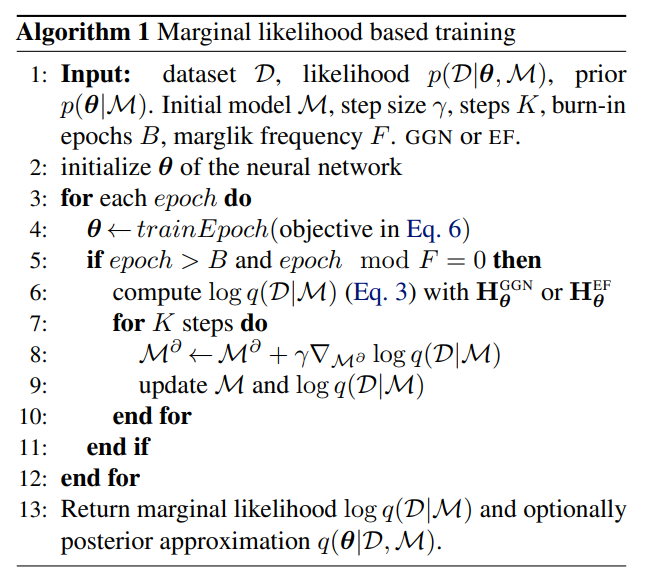
\includegraphics[scale=0.7]{images/img_algorithm.png}
    \end{figure}
\end{frame}

\section{Experiments}
\begin{frame}{Example approximation}
    \begin{figure}
        \centering
        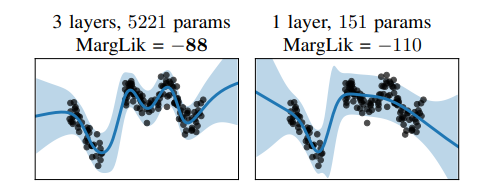
\includegraphics[scale=0.85]{images/example_1.png}
        \caption{A deeper 3-layer network (left) has a better
                marginal likelihood compared to a 1-layer network (right).
                This agrees with the fit where the deeper network appears to
                explain the ‘sinusoidal’ trend better.}
        \label{fig:enter-label}
    \end{figure}
\end{frame}

\begin{frame}{The connection between accuracy and MargLik}
    \begin{figure}
        \centering
        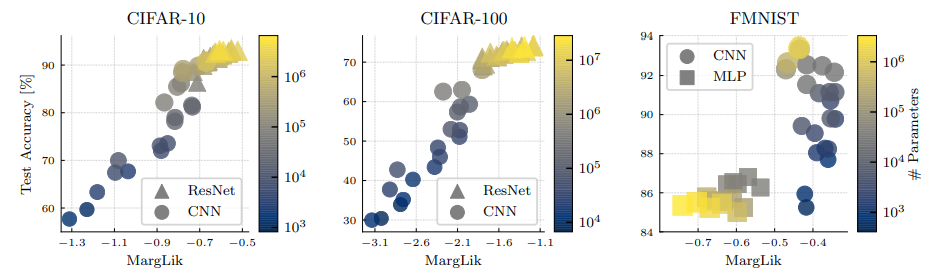
\includegraphics[scale=0.6]{images/example_2.png}
        \caption{Each dot above shows a model of different size and/or architecture (around 40 models per plot of varying widths and depths). Models with higher training marginal-likelihood tend to have higher test accuracy. For similar performance, smaller models tend to have a higher marginal-likelihood as desired. Marker size and color changes with the number of parameters.}
        \label{fig:enter-label}
    \end{figure}
\end{frame}

\section{Literature}
\begin{frame}{Literature}
    \begin{enumerate}
        \item \textbf{Main article} \href{https://proceedings.mlr.press/v139/immer21a/immer21a.pdf}
        {Scalable Marginal Likelihood Estimation for Model Selection in Deep Learning}.
    \end{enumerate}
\end{frame}

\end{document}